\documentclass[a4paper,8pt,french,fleqn]{article}
%Packages:

%Langages:
\usepackage[french]{babel}
\usepackage{lmodern}
\usepackage[T1]{fontenc}
\usepackage[utf8]{inputenc}

%AMS maths
\usepackage{amsmath, amssymb, amsfonts}

%Mise en page
\usepackage[top=3cm, right=2.5cm, bottom=3cm, left=2.5cm]{geometry}
\usepackage{fancyhdr}
\usepackage{enumerate}
\usepackage{color}
%Définition des macros
\usepackage{amsthm}

%Figures
\usepackage{tikz}
\usetikzlibrary{automata, positioning}

\usepackage{graphicx}
\usepackage{wrapfig}

%Symboles mathématiques
\usepackage{latexsym}

%Titre et auteurs

\title{\textbf{Projet Sudoku}\\\textit{Rapport du travail fourni}}
\author{PHILIPPI Alexandre \& HBAIEB Ahmed \& JEANJEAN Vincent}
\date{\today}

\begin{document}

\begin{figure}[h]
  \begin{center}
    
\includegraphics[scale=1.5]{enseirb.jpg}
    \vspace{2cm}
    \maketitle    
  \end{center}
\end{figure}

\newpage

\tableofcontents

\newpage

\section{Introduction}

Le but du projet était de réaliser un programme mettant en équation en logique propositionelle une grille de sudoku pour que le solveur SAT glucose puisse les résoudre. Le programme devait ensuite récupérer les informations renvoyées par glucose pour afficher la grille résolue si celle-ci était solvable. \\

Dans le cadre de ce projet, notre étude portait sur quatre grilles différentes de sudokus : classique / jigsaw / killer / comparison. Chacune de ces grilles était définie dans un fichier texte par un nombre de symboles, de lignes, de colonnes, un nom et des régles d'unicité, d'ordre et de somme. \\

Dans un premier temps, le programme réalisé devait permettre la résolution de grille de taille au plus $9 \times 9$. Puis dans un second temps il fallait l'adapter pour qu'il puisse permettre la résolution de grille de taille $n \times n$. Le programme devait aussi pouvoir assurer que les résultats renvoyés par le solveur SAT glucose respectaient bien les régles associées à la grille. 

\vspace{0.5cm}

\begin{figure}[h]
  \begin{center}
    \vspace{0.5cm}
    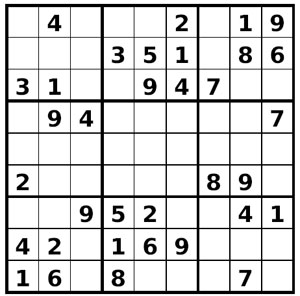
\includegraphics[scale=0.6]{sudoku.jpg}
    \hspace{1.5cm}
    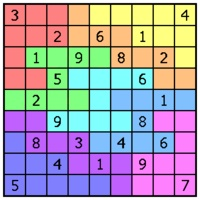
\includegraphics[scale=0.88]{jigsaw.jpg}
    \caption{Sudoku Classique \& Sudoku Jigsaw}
  \end{center}
\end{figure}

\begin{figure}[h]
  \begin{center}
    \vspace{0.5cm}
    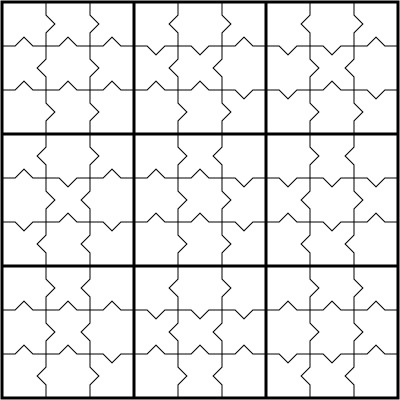
\includegraphics[scale=0.45]{comparison.jpg}
    \hspace{1.5cm}
    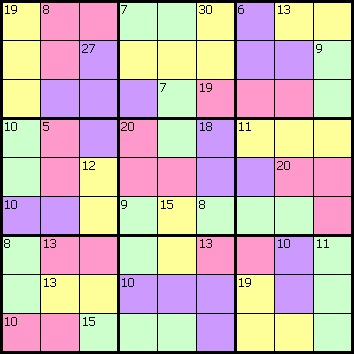
\includegraphics[scale=0.50]{killer.jpg}
    \caption{Sudoku Comparison \& Sudoku Killer}
  \end{center}
\end{figure}

\newpage

\section{Description de notre démarche}

Tout d'abord nous nous sommes concentrés sur la réalisation d'un automate capable de lire une grille et ses régles : 

  \begin{center}
    \begin{tikzpicture}[scale=0.2]
      \tikzstyle{every node}+=[inner sep=0pt]
      \draw [black] (11.1,-22.7) circle (3);
      \draw (11.1,-22.7) node {$q_1$};
      \draw [black] (25.1,-27.5) circle (3);
      \draw (25.1,-27.5) node {$q_2$};
      \draw [black] (14.3,-45.5) circle (3);
      \draw (14.3,-45.5) node {$q_6$};
      \draw [black] (36.8,-49.9) circle (3);
      \draw (36.8,-49.9) node {$q_7$};
      \draw [black] (37.9,-21.6) circle (3);
      \draw (37.9,-21.6) node {$q_3$};
      \draw [black] (50.8,-21.6) circle (3);
      \draw (50.8,-21.6) node {$q_4$};
      \draw [black] (25.1,-11) circle (3);
      \draw (25.1,-11) node {$q_5$};
      \draw [black] (52.2,-47.7) circle (3);
      \draw (52.2,-47.7) node {$q_8$};
      \draw [black] (39.1,-37.4) circle (3);
      \draw (39.1,-37.4) node {$q_9$};
      \draw [black] (13.94,-23.67) -- (22.26,-26.53);
      \fill [black] (22.26,-26.53) -- (21.67,-25.79) -- (21.34,-26.74);
      \draw (16.66,-25.65) node [below] {$'s'$};
      \draw [black] (11.52,-25.67) -- (13.88,-42.53);
      \fill [black] (13.88,-42.53) -- (14.27,-41.67) -- (13.28,-41.81);
      \draw (12.01,-34.27) node [left] {$'o'$};
      \draw [black] (17.24,-46.08) -- (33.86,-49.32);
      \fill [black] (33.86,-49.32) -- (33.17,-48.68) -- (32.97,-49.66);
      \draw (20.21,-49.07) node [below] {$'\textbf{\textvisiblespace}([1...9]^*,[1...9]^*)\textbf{\textvisiblespace}'$};
      \draw [black] (25.663,-24.572) arc (-201.98248:-288.52403:7.747);
      \fill [black] (35.31,-20.13) -- (34.71,-19.4) -- (34.39,-20.35);
      \draw (24.1,-19.89) node [above] {$'\textbf{\textvisiblespace}[1...9]^*\textbf{\textvisiblespace}('$};
      \draw [black] (49.871,-24.424) arc (-31.48538:-148.51462:6.474);
      \fill [black] (49.87,-24.42) -- (49.03,-24.85) -- (49.88,-25.37);
      \draw (44.35,-28.02) node [below] {$'[1...9]^*,[1...9]^*)\textbf{\textvisiblespace}'$};
      \draw [black] (11.811,-19.788) arc (162.03676:21.13751:20.233);
      \fill [black] (11.81,-19.79) -- (12.53,-19.18) -- (11.58,-18.87);
      \draw (30.47,-5.26) node [above] {$'*'$};
      \draw [black] (40.176,-19.67) arc (119.99867:60.00133:8.348);
      \fill [black] (40.18,-19.67) -- (41.12,-19.7) -- (40.62,-18.84);
      \draw (44.35,-18.05) node [above] {$'('$};
      \draw [black] (13.4,-20.78) -- (22.8,-12.92);
      \fill [black] (22.8,-12.92) -- (21.86,-13.05) -- (22.5,-13.82);
      \draw (16.34,-16.36) node [above] {$'u'$};
      \draw [black] (27.969,-11.864) arc (68.43967:32.30232:17.89);
      \fill [black] (36.52,-18.94) -- (36.51,-18) -- (35.67,-18.53);
      \draw (34.61,-14.23) node [above] {$'\textbf{\textvisiblespace}('$};
      \draw [black] (39.77,-49.48) -- (49.23,-48.12);
      \fill [black] (49.23,-48.12) -- (48.37,-47.74) -- (48.51,-48.73);
      \draw (45.78,-49.65) node [below] {$'>','<'$};
      \draw [black] (49.84,-45.85) -- (41.46,-39.25);
      \fill [black] (41.46,-39.25) -- (41.78,-40.14) -- (42.4,-39.36);
      \draw (55.46,-42.05) node [above] {$'\textbf{\textvisiblespace}([1...9]^*,[1...9]^*)\textbf{\textvisiblespace}'$};
      \draw [black] (36.227,-38.254) arc (-77.51136:-157.88758:21.176);
      \fill [black] (12.03,-25.55) -- (11.87,-26.48) -- (12.79,-26.1);
      \draw (20.21,-36.83) node [below] {$'*'$};
    \end{tikzpicture}
  \end{center}

Nous avons ensuite cherché à comprendre le fonctionnement de la logique propositionnelle et de glucose à l'aide d'une grille de taille $2 \times 2$ et une fois le principe compris, nous nous sommes occupés de la mise en équation de la grille de sudoku classique de taille $9 \times 9$. \\

Puis nous avons réalisé l'automate utilisé pour lire le retour de glucose et afficher la grille résolue dans le terminal pour s'assurer que la grille résolue était juste. \\

Nous avons ensuite réalisé les fonctions mettant en équation les autres grilles excepté la grille du sudoku killer que nous avons tenté de faire à la fin. Puis pour s'assurer que les résultats étaient juste sans avoir à refaire soi-même les grilles nous avons développé une fonction permettant de vérifier que les régles de la grille étaient respectées. \\

Finalement, nous avons élargi le champs d'action de notre programme pour des grilles de taille $n \times n$ avec n tel qu'on ait à faire à un carré magique. \\

\newpage

\section{Solution employée}

\subsection{Lecture grille}

Pour la lecture de la grille et de ses régles nous avons opté pour la programmation d'un automate. C'est une solution plus longue à coder qu'un simple enchaînement de fonction 'fscanf' mais elle permet de localiser plus facilement une erreur de formatage dans le fichier associé à la grille puisque celui-ci est lu caractère par caractère.

\subsection{Traduction grille}

Pour la mise en équation en logique propositionelle de la grille nous avons eu à distinguer chaque type de grilles : \\

\subsubsection*{Sudoku classique}

Les régles du sudoku classique impose que dans chaque lignes, chaque colonnes, et chaque régions, la valeur dans une cellule soit unique. Les équations logiques associées correspondent donc à une suite d'implications entre deux cellules. On pose l'inconnu $p_{ijk}$ qui signifie : dans la cellule de coordonnées (i,j) se trouve la valeur k. Une implication serait : $p_{111} \Rightarrow \neg p_{121}$ ce qui donne en logique propositionelle : $-111 \lor -121$. Pour écrire toutes les équations nous avons donc décidé de réaliser une fonction qui balaye la grille entièrement et qui pour chaque valeur dans chaque cellule écrit l'implication associée avec chaque autres cellules de la ligne, de la colonne et de la région.

\subsubsection*{Sudoku jigsaw}

La seule en différence entre le sudoku jigsaw et le classique est la forme des régions. Les sous-groupes ne sont plus de simples carrés mais des formes géométriques plus complexes. Cependant en soit, la traduction en équations reste la même.

\subsubsection*{Sudoku comparison}

La grille du sudoku comparison correspond à une grille vide, avec des symboles d'inégalités entre chaque cellules. Ainsi en plus des régles du sudoku classique à respecter, les inégalités entre chaques cellules doivent l'être aussi. Si par exemple entre la cellule de coordonnées (1,1) et celle de cordonnées (1,2) il y a un symbole '>' deux des équations de logique propositionelle seraient : $ -115 \lor -126$ et $-128 \lor -117$. Il y a donc des équations à rajouter en plus de celles du sudoku classique, les équations traduisant les inégalités, pour ce faire nous avons réalisé une boucle balayant toutes les valeurs dans toutes les cellules et écrivant les implications associées en fonction des valeurs de chaque cellules et des inégalités.

\subsubsection*{Sudoku killer}

La grille du sudoku killer est une grille de sudoku classique à laquelle on ajoute des règles sur un groupement de cellules. Ces règles sont de types somme et unicité chaque groupement de cellules aura une valeur associée correspondant à la somme des valeurs des trois cellules, les régles d'unicité seront elles entre différentes cellules de la grille de sudoku. Les régles d'unicité sont mises en équations grâce à la même fonction que celle du jigsaw. Pour la mise en place des équations associées aux régles de sommes nous avons du faire face à quelques problèmes. Nous nous sommes intéressés aux combinaisons possibles pour chaque groupement de cellules en fonction de la valeur de la somme et du nombre de cellules. Pour cela, nous avons pensé à une boucle de longueur variable mise en place grâce à un appel récursif. (Cette idée a été testée et a fait l'objet d'une recherche infructueuse) 

\subsection{Lecture des résultats de Glucose}

Encore une fois, pour lire le fichier texte contenant le retour de glucose la solution choisie a été un automate. Pour les mêmes raisons qu'énoncées précédemment, l'automate évite de perdre du temps pour savoir où est localisée l'erreur de formatage du fichier, et c'est un outil qui donne plus de clarté au code. Pour récupérer les données de glucose, nous avons redirigé son flux vers un fichier texte. Il faut savoir que glucose renvoit 3 types de lignes, les lignes 'c' pour commentaire, 's' pour savoir si le problème est 'satisfiable' et 'v' pour les résultats. Notre automate, lors de la lecture du fichier néglige toutes les lignes commençant par un 'c'. Puis il vérifie que le problème est 'satisfiable', si tel est le cas, il lit les résultats en négligeant tous les résultats commençant par un '-'.

\subsection{Validation de la grille}

Pour valider les informations renvoyées par glucose, les résultats obtenus doivent être comparés avec les régles de chaque grille : \\

\subsubsection*{Sudoku classique}

Pour vérifier la validité de la grille, on utilise une fonction simple réalisant une comparaison entre une case fixée (que nous faisons varier pour balayer toute la grille) et les autres cases sur la même ligne que la case, sur la même colonne et sur le même groupement de cellules. La fonction crée a pour but de vérifier si un symbole ne réapparait pas plusieurs fois sur les règles d'unicités propres au sudoku. Cette solution n'est pas optimale d'un point de vue complexité car elle demande un nombre très élevé de calculs et effectue un certains nombre de calculs plusieurs fois. Un tri par insertion par exemple aurait été plus avantageux et plus rapide que notre méthode.   

\subsubsection*{Sudoku jigsaw}

On réalise la même démarche que pour le sudoku classique.

\subsubsection*{Sudoku comparison}

On réalise la même démarche que pour le sudoku classique et on réalise une vérification supplémentaire pour les inégalités.

\subsubsection*{Sudoku killer}

On réalise la même démarche que pour le sudoku classique en rajoutant les vérifications sur les sommes des groupements cellules ``somme'' et les vérifcations sur les groupements ``unicité''.

\subsection{Affichage de la grille}

L'affichage de la grille avant et aprés résolution se fait dans le terminal. Par manque de temps nous n'avons pas pu développer une fonction créant un fichier au format '.pdf'.

\subsection{Grille de taille $n \times n$}

Pour adapter notre programme à des grilles de taille $n \times n$ tel qu'on ait un carré magique nous avons joué sur le changement de base pour l'écriture des coordonées des cellules. Ainsi pour une grille de taille 'nsymbols' nous avons dit que par exemple la cellule de coordonnées (1,1) avec la valeur 1 donné 111 dans la base $nsymbols + 1$. Avant d'envoyer la valeur à glucose nous convertissions donc celle-ci dans la base décimale. Ensuite, une fois les valeurs récupérées en sortie de glucose il ne nous restait plus qu'à reconvertir la valeur dans la base $nsymbols + 1$.

\newpage

\section{Autour des algorithmes}

\subsection{Choix}

Pour répondre au sujet, notre recherche s'est avant tout portée sur des grilles de dimension au plus $9 \times 9$. Pour la traduction des grilles nous n'avons pas cherché à faire un algorithme optimisé s'exécutant rapidement. C'est pourquoi nous avons opté pour des algorithmes basiques, simples à mettre en place mais de complexité en temps très élevé. Pour tous les sudokus nous avons donc réalisé des algorithmes balayant toutes les cellules, pour toutes les valeurs, écrivant à chaque fois les implications entre chaque cellule pour toutes les régles, quitte à avoir des doublons au niveau des équations écrites dans le fichier envoyé au solveur SAT.

\subsection{Complexité}

\subsubsection*{Sudoku classique}

Comme dit précédemment nous n'avons pas cherché à faire un algorithme optimal au niveau complexité temporelle et spatiale. \`A  la place nous avons opté pour un algorithme simple à écrire mais réalisant un nombre d'actions très élevé, ce qui nous amène à une complexité en temps de :\\
 
\begin{itemize}
  
\item $nsymbol \times nrows \times ncolumns \times \sqrt{nrows} \times \sqrt{ncolumns}$ pour les régions ; \\
  
\item $nsymbol \times nrows \times ncolumns \times nrows$ pour les équations liées au lignes ; \\

\item $nsymbol \times nrows \times ncolumns \times ncolumns$ pour les équations liées aux colonnes ; \\

\item $nsymbols \times nrows \times ncolumns$ pour les équations associées à chaque cellules (pour forcer la présence d'une valeur) ;\\

\end{itemize}

C'est à dire si les paramètres de la grille ont la même valeur 'n' : $3 \times n^{4} + n^{3}$. 

\subsubsection*{Sudoku jigsaw}

Pour le sudoku jigsaw, la complexité en temps est la même que pour le sudoku classique, car il possède les mêmes régles. Le seul changement intervient dans la forme des groupements de cellules qui ne sont plus des carrés de taille $\sqrt(nsymbols) \times \sqrt(nsymbols)$ mais des formes géométriques particulières qui contiennent aussi nsymbols.

\subsubsection*{Sudoku comparison}

Pour le sudoku comparison, on utilise les mêmes algorithmes que dans le sudoku classique, plus un algorithme pour mettre en équation les inégalités entre chaque cellules voisines d'une même région qui est de complexité : \\

\begin{itemize}

\item $nb\_relations \times nsymbols \times nsymbols \times 2$, le facteur 2 correspond aux implications réciproques ;\\

\end{itemize}

On a donc au final une complexité de la forme : $3 \times n^{4} + 3 \times n^{3}$. 

\subsubsection*{Sudoku killer}

La complexité de ce type de sudoku se révèle être la plus élevée car elle comprend la complexité du sudoku classique, plus la mise en place des régles d'unicité particulières, plus la recherche de toutes les sommes possibles pour obtenir la valeur associée à chaque sous-groupes de cellules. On trouve alors en complexité, pour une somme avec 'k' cases : \\

\begin{itemize}

\item $nsymbols^{k}$ \\

\end{itemize}  

Cependant, si on compte toutes les opérations effectuées lors de la retranscription des données au format DIMACS, on obtient une complexité de l'ordre de:\\

\begin{itemize}

\item $\Sigma_{k=2}^{n} nb\_sommes_k \times nsymbols^{k} + Complexité(sudoku\_classique)$ où la première somme correspond à la complexité issue de la recherche des combinaisons possibles pour chaque ``groupement de cellules somme'' \\

\end{itemize}

On se retrouve donc avec une complexité en espace et en temps beaucoup plus importante que pour les autres types de sudoku.

\subsection{Problèmes rencontrés}

Un problème majeur pour notre groupe a été la compréhension du fonctionnement des équations à envoyer à glucose. Nous avons perdu beaucoup de temps à comprendre comment le format 'dimacs' fonctionnait, et quelles équations nous allions réaliser pour permettre à glucose de résoudre les grilles. Cependant, l'essai sur une grille de taille $2 \times 2$ nous a permis de mieux comprendre le principe.

Une fois le principe compris, il ne restait plus qu'à comprendre les régles particulières à chaque grilles. Cependant la grille du sudoku killer a été pour nous un véritable de défi que nous n'avons pas su résoudre malgré de nombreuses idées qui nous amenaient toujours à recevoir de glucose la même réponse : 'unsatisfiable'. Malgré tout, nous avons eu une dernière idée que nous n'avons pas eu le temps de mettre en place mais qui a été précisé un peu plus haut. \\

Un problème majeur rencontré lors de la création de notre programme est la mise en place des équations pour le sudoku killer. Nous n'avons pas réussi à exprimer celà de manière correcte pour que celà puisse être envoyé au solveur Sat-Glucose. Cependant, afin de ne pas provoquer de problèmes au niveau du fonctionnement du programme, nous avons décidé de bloquer la partie concernant le sudoku killer.\\ 

Enfin, le dernier problème majeur venait des grilles de tailles trop grandes ou bien, avec trop peu de données, notamment pour le sudoku classique. En effet, la taille du sudoku et le nombre de valeurs présentes intialement présente dans la grille peuvent provoquer un ``UNSATISFIABLE'' (dans le cas où il n'y a pas de solutions viables) ou bien un ``INDETERMINATE'' (cas où le solveur n'a pas assez d'équations). Ce dernier cas n'est apparu que pour des grandes grilles (de taille supérieure ou égale à $36 \times 36$) et peu remplies. Il s'avère cependant que, pour des grilles de sudokus classiques (de taille inférieure à $36 \times 36$) avec aucune valeur présente initialement dans la grille, le solveur SAT glucose est capable de trouver une solution (parmis un grand nombre). 


\subsection{Améliorations envisageables}

Beaucoup de choses nécessitent des améliorations dans notre programme. Tout d'abord, il serait bon de réaliser une fonction écrivant dans un fichier '.tex' la grille avant et aprés résolution pour la rendre plus lisible. C'était l'un de nos objectifs mais par manque de temps nous n'avons pas pu le valider. Nous pourrions aussi améliorer nos algorithmes pour faire en sorte de réduire au maximum le nombre d'équations envoyées à glucose notamment en supprimant tous les doublons et en cherchant peut être une meilleure méthode. Par ailleurs, ceci permettrait peut-être d'améliorer la résolution des sudoku pour des tailles plus grandes. De plus, afin d'améliorer notre programme, nous pourrions mettre en place des stratégies de résolution en fonction des cases déjà présentes, ce qui permettrait de réduire considérablement le nombre d'équations envoyées au glucose. La taille des grilles gérées pourrait alors augmenter. (On peut espérer résoudre des grilles de taille $100 \times 100$ par cette méthode). \\

Enfin, pour le sudoku killer, qui correspond à notre point noir du point de vue de la complexité, il pourrait s'agir de faire appel à d'autres programmes, plus performants, afin de trouver les combinaisons possibles pour ``les groupements de sommes'' ou tout simplement, stocker les combinaisons dans un fichier ``.txt'' et aller régulièrement piocher dedans afin de mettre en place les équations en logique propositionnelle. Ceci réduirait le temps d'exécution du programme de manière considérable.

\section{Conclusion}

Finalement, nous avons quand même réalisé la majorité des objectifs fixés pour ce projet. A travers ce premier projet d'informatique nous avons pu remarquer l'importance de la communication au sein d'un groupe ainsi que la bonne répartition des tâches pour que le projet avance bien, et que les idées convergent vers un même point. 

\end{document}
